For testing purposes, the project was deployed on the developer's local machine. Initially the application was run straight out of the IDE, but docker instructions for deploying the models were written as well, to simplify deployment in a cloud environment.

\subsection{Deploying the API Server}

For deploying the server on your local machine, first clone the root repository (that contains this report) to your drive. Cloning to a Windows DEV Drive is recommended to increase performance.

Ensure that Python \texttt{3.11.9} is installed on your computer. We believe that any 3.11.* version should work, but it has not been tested. Proceed at your own risk. Python 3.12 will NOT work. Don't even try.

Navigate to the \texttt{src/api-server} folder, and open a terminal there.

First, you will have to create a new virtual environment. This is to containerize your packages, so that it doesn't mess with other projects or your systemwide python installation. In this example, \texttt{testenv} is used as the environment name as this is a testing deployment.
\begin{verbatim}
    python -m venv testenv
\end{verbatim}

Next, activate the newly created venv. This script is for windows installations only.
\begin{verbatim}
    .\venv\Scripts\activate
\end{verbatim}
The activation script is different on other operating systems, please consult the documentation for venv for your operating system version to determine the correct syntax.

Then, install all necessary modules.
\begin{verbatim}
    pip install -r .\requirements.txt
\end{verbatim}

Before running the server, you can configure what models are available for use by server. Go to \texttt{app.py}, and add or remove available models from line 16 onwards. We recommend not enabling the BERT based models unless you know what you're doing, and have a powerful computer.

Finally, run the flask server.
\begin{verbatim}
    flask run
\end{verbatim}

If you wish to use Docker, a Dockerfile is available in the root directory of the api-server project. Run it on your server of choosing.

\subsection{Deploying the Demo Application}

For testing purposes, we recommend running the app locally. To do so, first clone the root repository (that contains this report) to your drive. As mentioned above, cloning to a Windows DEV Drive will increase compile perfomance.

You will need \texttt{nodejs} and \texttt{npm} installed. Please refer to the offical documentation for instructions on how to install node and npm.

Start by opening up a terminal in the \texttt{src/api-demo-app} folder. Update packages by running
\begin{verbatim}
    npm install
\end{verbatim}

Next, run the development server by running,
\begin{verbatim}
    npm run dev
\end{verbatim}

Your development server is now running, and you should be able to access the page.

NOTE: The application will not function unless the api-server is also running, for obvious reasons. As far as our testing goes, we ran the api-server on port 5000, and the demo server on port 3000.

We intend to deploy the api-demo-server on Vercel, for it's ease of use and compatibility with Github for CI/CD pipelines.

\begin{figure}[htbp]
    \centering
    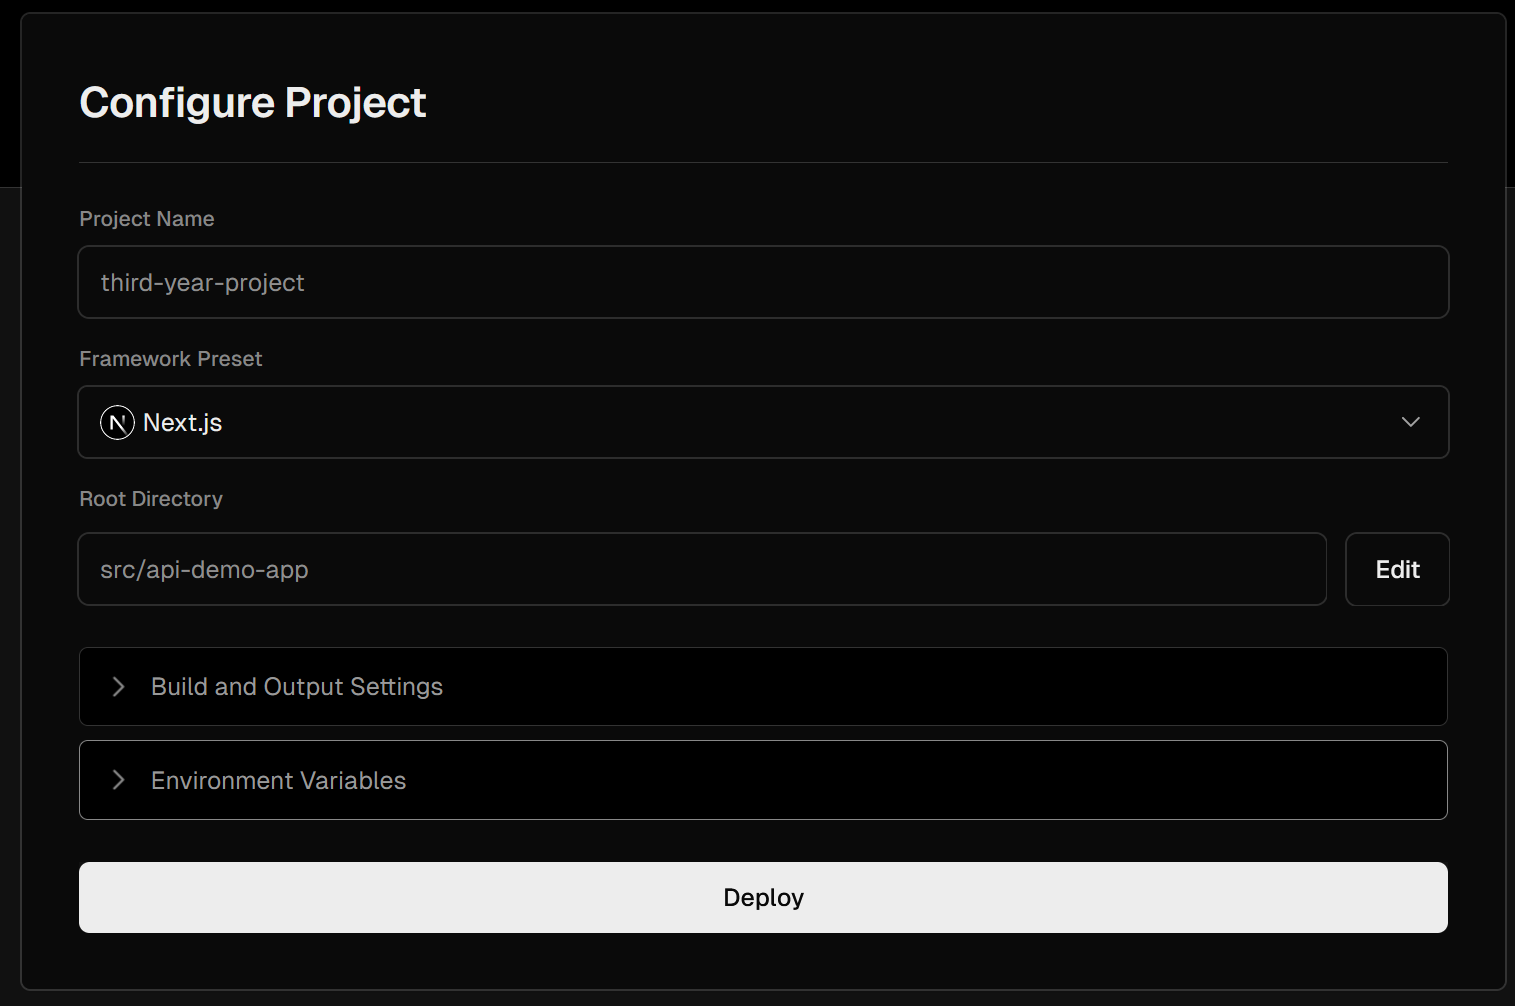
\includegraphics[width=1\textwidth]{../../assets/vercel_deployment.png}
    \caption{Settings used in deploying the application}
    \label{fig:configuration}
\end{figure}

Deployment is done on Vercel by first creating an account, giving conditional access to the repository to be deployed (ThirdYearProject in this case), selecting the root directory, and deploying the application. The production deployment is sourced from the main branch, and active development is conducted on other branches, and merged with the main branch.